En esta sección se explicará el diseño final del modelo de datos que se utilizará en el sistema.  Para facilitar la lectura se dividirá en dos partes: una parte mostrará el modelo relativo a la zona de datos (subsistema de datos) y la otra mostrará el modelo utilizado en la zona social (subsistemas de gestión de usuarios, debates, noticias, eventos, etc).


\subsection{Modelo de la zona de datos}
\label{modelo_datos_zona_datos}
\subsubsection{Diagrama del modelo de datos}
La figura \ref{fig:diagrama_modelo_final} muestra el diagrama con el diseño final del modelo del subsistema de datos.
\begin{landscape}
	\begin{figure}[h]
		\centering
		\includegraphics[width=25cm]{arquitectura/modelo}
		\caption{Diseño final del modelo de datos}
		\label{fig:diagrama_modelo_final}
	\end{figure}
\end{landscape}

Como se puede comprobar, existe una variación importante respecto a lo originalmente diseñado en la figura \ref{fig:clases_preliminares_modelo_book} perteneciente a la sección ``\nameref{clases_preliminares_modelo_datos}'' del capítulo \ref{chapter04}.  A continuación se expondrán las razones para ésta divergencia:

\paragraph{Especificación más cercana al RDF Data Cube Vocabulary} \hfill \\
Como se explicó anteriormente en el capítulo \ref{chapter03}, el RDF Data Cube Vocabulary organiza las observaciones en torno a un grupo de \textit{dimensiones}, \textit{medidas} y \textit{atributos}.

Para dar soporte a ésto se han incluido la clase ``\textit{Dimension}'', de la que heredarán todas las dimensiones, las clases ``\textit{MeasurementUnit}`` y ``\textit{Value} pretenden dar entidad completa a las medidas y, por último, las clases ``\textit{Computation}'' y ``\textit{Time}'' pretenden dar entidad a los atributos de las observaciones.

También se ha incluido soporte a slices con la clase ``\textit{Slice}''.

\paragraph{Inclusión de soporte para la internacionalización de datos} \hfill \\
Tal y como se definió en el requisito \textit{RLB 7} en la sección ``\nameref{requisitos_seccion_datos}'' del capítulo \ref{chapter04}, es necesario soportar la internacionalización en el nivel de datos.

Éste soporte ha sido incluido con las clases ``\textit{Language}``, ``\textit{OrganizationTranslation}``, ``\textit{RegionTranslation}``, ``\textit{TopicTranslation}`` e ``\textit{IndicatorTranslation}``.

\paragraph{Soporte a distintos intervalos temporales} \hfill \\
Puesto que las observaciones pueden hacer referencia a diferentes intervalos temporales, se han incluido las clases ``\textit{Interval}'', ``\textit{YearInterval}'' y ``\textit{MonthInterval}''.

\subsubsection{Elementos del modelo de datos}
A continuación se explicará el cometido de cada una de las clases del modelo que se han mostrado en la figura \ref{fig:diagrama_modelo_final}.

\begin{description}
	\item[Language]  Representa un idioma en el que se traducirán los datos.  Sus atributos son los siguientes:
		\begin{itemize}
			\item \textbf{Lang code}  Código de dos letras del idioma
			\item \textbf{Name}  Nombre del idioma
		\end{itemize}
	\item[RegionTranslation]  Traduce el nombre de una región.  Sus atributos son los siguientes:
		\begin{itemize}
			\item \textbf{Lang code}:  Código del idioma en el que se almacena la traducción
			\item \textbf{Region id}:  Identificador único de la región para la cual se almacena la traducción
			\item \textbf{Name}:  Nombre traducido de la región en el idioma correspondiente
		\end{itemize}
	\item[User]  Representa a un usuario que incluye información en el sistema (un importador).  Sus atributos son los siguientes:
		\begin{itemize}
			\item \textbf{Id}:  Identifica de forma única a cada usuario
			\item \textbf{IP}:  Dirección IP desde la que se realiza la petición de importación de datos
			\item \textbf{Timestamp}:  Momento temporal en el que se recibe la petición de importación de datos
			\item \textbf{Organization id}:  Identificador de la organización a la que pertenece el importador
		\end{itemize}
	\item[Organization]  Representa a una organización de la cual se incluyen datos en el sistema.  Sus atributos son los siguientes:
		\begin{itemize}
			\item \textbf{Id}:  Identifica de forma única a cada organización
			\item \textbf{Name}:  Es el nombre de la organización
			\item \textbf{URL}:  Dirección del sitio web de la organización
			\item \textbf{Is part of id}:  Identificador de la organización a la que pertenece (en el caso de que pertenezca a alguna)
		\end{itemize}
	\item[DataSource]  Representa una fuente de datos que aporta información al sistema.  Sus atributos son los siguientes:
		\begin{itemize}
			\item \textbf{Id}:  Identifica de forma única a cada fuente de datos
			\item \textbf{Name}:  Es el nombre de la fuente de datos
			\item \textbf{Organization id}:  Identificador de la organización a la que pertenece la fuente de datos
		\end{itemize}
	\item[DataSet]  Representa un conjunto de datos que se ha incluido en el sistema.  Sus atributos son los siguientes:
		\begin{itemize}
			\item \textbf{Id}:  Identifica de forma única a cada fuente de datos.
			\item \textbf{Sdmx frequency}:  Frecuencia con la cual la fuente actualiza sus datos.  Los valores para este campo son tomados de la ontología SDMX\footnote{Para más información véase \url{http://publishing-statistical-data.googlecode.com/svn/trunk/specs/src/main/vocab/sdmx-code.ttl}}
			\item \textbf{Datasource id}:  Identificador de la fuente de datos a la que pertenece éste conjunto de datos
			\item \textbf{License id}:  Identificador de la licencia bajo la que se publica éste conjunto de datos
			\item \textbf{Indicators}: Indicadores con los que cuenta la fuente de datos.
		\end{itemize}
	\item[OrganizationTranslation]  Almacena los datos de una organización en diferentes idiomas.  Sus atributos son los siguientes:
		\begin{itemize}
			\item \textbf{Lang code}:  Código del idioma en el que se almacena la traducción
			\item \textbf{Organization id}:  Identificador único de la organización para la cual se almacena la traducción
			\item \textbf{Description}:  Descripción traducida de la organización en el idioma correspondiente
		\end{itemize}
	\item[Slice]  Representa una slice\footnote{El concepto de slice fue explicado en la sección ``\nameref{concept:rdf_data_cube}'' del capítulo \ref{chapter03}}.  Sus atributos son los siguientes:
		\begin{itemize}
			\item \textbf{Id}:  Identificador único de la slice
			\item \textbf{Indicator id}:  Identificador único del indicador con el cual se relaciona el slice
			\item \textbf{Dimension}:  Identificador único de la otra dimensión con la que se relaciona el slice (o bien una región o bien un momento temporal)
			\item \textbf{Dataset id}:  Identificador único del conjunto de datos del que procede la slice
		\end{itemize}
	\item[Observation]  Representa una observación para un indicador y una región en un determinado momento temporal.  Sus atributos son los siguientes:
		\begin{itemize}
			\item \textbf{Id}:  Identificador único de la observación
			\item \textbf{Ref time id}:  Identificador único del momento temporal al que la observación hace referencia
			\item \textbf{Issued id}:  Identificador único del momento temporal en el que la observación fue incluida en el sistema
			\item \textbf{Computation id}:  Identificador único de la computación con la que se relaciona la observación
			\item \textbf{Indicator group id}:  Identificador único del grupo de indicadores con el que se relaciona la observación (si se relaciona con alguno)
			\item \textbf{Value id}:  Identificador único del valor de la observación
			\item \textbf{Indicator id}:  Identificador único del indicador al que pertenece la observación
			\item \textbf{Dataset id}:  Identificador único del conjunto de datos al que pertenece la observación
			\item \textbf{Region id}:  Identificador único de la región a la que hace referencia la observación
			\item \textbf{Slice id}:  Identificador único del slice al que pertenece la observación (en caso de pertencer a alguno)
		\end{itemize}
	\item[Indicator]  Representa un indicador sobre el cual se realizan mediciones.  Sus atributos son los siguientes:
		\begin{itemize}
			\item \textbf{Id}:  Identificador único del indicador
			\item \textbf{Preferable tendency}:  Representa la tendencia preferible del indicador a lo largo del tiempo
			\item \textbf{Measurement unit id}:  Identificador único de la unidad de medida para los valores de las observaciones del indicador
			\item \textbf{Compound indicator id}:  Identificador del indicador compuesto con el que se relaciona el indicador (en caso de relacionarse con alguno)
			\item \textbf{Last update}:  Fecha de la ultima actualización del indicador o alguna de sus observaciones en el sistema
			\item \textbf{Starred}:  Indica si el indicador ha sido marcado como favorito o no
			\item \textbf{Topic id}:  Identificador único del tópico al que pertenece el indicador
		\end{itemize}
	\item[IndicatorTranslation]  Almacena los datos de un indicador en diferentes idiomas.  Sus atributos son los siguientes:
		\begin{itemize}
			\item \textbf{Lang code}:  Código del idioma en el que se almacena la traducción
			\item \textbf{Indicator id}:  Identificador único del indicador para el cual se almacena la traducción
			\item \textbf{Name}:  Nombre del indicador traducido en el idioma correspondiente
			\item \textbf{Description}:  Descripción del indicador traducida en el idioma correspondiente
		\end{itemize}
	\item[Topic]  Representa un tópico sobre el cual se guardan indicadores.  Su único atributo es un código que lo identifica.
	\item[TopicTranslation]  Almacena los datos de un tópico en diferentes idiomas.  Sus atributos son los siguientes:
		\begin{itemize}
			\item \textbf{Lang code}:  Código del idioma en el que se almacena la traducción
			\item \textbf{Indicator id}:  Identificador único del tópico para el cual se almacena la traducción
			\item \textbf{Name}:  Nombre del tópico traducido en el idioma correspondiente
		\end{itemize}
	\item[IndicatorGroup]  Representa una agrupación de indicadores compuestos.  Su único atributo es un código que lo identifica.
	\item[MeasurementUnit]  Representa a una unidad de medida.  Sus atributos son los siguientes:
		\begin{itemize}
			\item \textbf{Id}:  Identificador único de la unidad de medida
			\item \textbf{Name}:  Nombre de la unidad de medida
			\item \textbf{Convertible to}:  Unidad estándar a la que es convertible\footnote{Por ejemplo: si la unidad de medida fueran centímetros, la unidad estándar a la que es convertible serían metros}
			\item \textbf{Factor}:  Factor de conversión a aplicar al valor para convertirlo a la unidad estándar
		\end{itemize}
	\item[License]  Representa una licencia bajo la cual se publica algún conjunto de datos almacenado en el sistema.  Sus atributos son los siguientes:
		\begin{itemize}
			\item \textbf{Id}:  Identificador único de la licencia
			\item \textbf{Name}:  Nombre de la licencia
			\item \textbf{Description}:  Descripción larga de la licencia
			\item \textbf{Republish}:  Indica si la licencia autoriza o no a republicar los datos
			\item \textbf{URL}:  Sitio web de la licencia
		\end{itemize}
	\item[Computation]  Representa una computación que se realiza sobre los valores de una observación.  Sus atributos son:
		\begin{itemize}
			\item \textbf{Id}:  Identificador único de la computación
			\item \textbf{Name}:  URL de la computación\footnote{Las URL de las computaciones son tomadas de la ontología WESO-Computex, para más información véase \url{https://raw.githubusercontent.com/weso/computex/master/ontology/computex.rdf}}
			\item \textbf{Description}:  Descripción de la computación
		\end{itemize}
	\item[Value]  Representa un valor de una observación.  Sus atributos son:
		\begin{itemize}
			\item \textbf{Id}:  Identificador único del valor
			\item \textbf{Obs status}:  Estado de la observación\footnote{Éste campo permite distinguir entre aquellas observaciones nulas y aquellas observaciones que no cuentan con un valor.  Ésta distinción es necesaria para asegurar la calidad estadística de los datos.}
			\item \textbf{Value}:  Almacena el valor concreto
			\item \textbf{Value type}:  Indica el tipo del valor almacenado
		\end{itemize}
	\item[IndicatorRelationship]  Representa una relación entre varios indicadores.  Su único atributo es un código que identifica la relación.  Existen dos tipos de relaciones:  \textbf{Becomes}, que representa un indicador que se transforma en otro a lo largo del tiempo y \textit{IsPartOf}, que representa un indicador que forma parte de otro
	\item \textbf{Dimension}:  Representa una dimensión tal y como se define en el \nameref{concept:rdf_data_cube}.  Su único atributo es un código que la identifica
	\item[Time]  Representa una unidad de tiempo.  Hereda los atributos de \textbf{Dimension}
	\item[Instant]  Representa un momento concreto en el tiempo.  Además de los atributos que hereda de \textbf{Time} también incluye:
	\begin{itemize}
		\item \textbf{Timestamp}:  Momento concreto en el tiempo al que hace referencia
	\end{itemize}
	\item[Interval]  Representa un intervalo arbitrario de tiempo.  Además de los atributos que hereda de \textbf{Time} también incluye:
	\begin{itemize}
		\item \textbf{Start time}:  Momento en el que comienza el intervalo de tiempo
		\item \textbf{End time}:  Momento en el que finaliza el intervalo de tiempo
		\item \textbf{Value}:  Valor del intervalo en forma de texto para su posterior presentación en las vistas
	\end{itemize}
	\item[YearInterval]  Representa un intervalo de un año.  Además de los atributos que hereda de \textbf{Interval} también incluye:
	\begin{itemize}
		\item \textbf{Year}:  Año concreto al que hace referencia el intervalo
	\end{itemize}
	\item[MonthInterval]  Representa un intervalo de un mes.  Además de los atributos que hereda de \textbf{Interval} también incluye:
	\begin{itemize}
		\item \textbf{Year}:  Año concreto al que hace referencia el intervalo
		\item \textbf{Month}:  Mes concreto al que hace referencia el intervalo
	\end{itemize}
	\item[Region]  Representa una región sobre la que se almacenan observaciones.  Además de los atributos que hereda de \textbf{Dimension} también tiene:
	\begin{itemize}
		\item \textbf{Un code}:  Será el código numérico asignado por la División Estadística de las Naciones Unidas\footnote{Éste código recibe el nombre formal de ``ISO 3166-1 numeric''.  En \cite{un:standard-country-codes} y \cite{un:iso-3166-country-codes} puede encontrarse más información sobre éstos códigos.} para la región
		\item \textbf{Is part of id}:  Identificador único de la región de la que forma parte (en caso de formar parte de alguna)
	\end{itemize}
	\item[Country]  Representa un país sobre el que se almacenan observaciones.  Además de los atributos que hereda de \textbf{Region} también tiene:
	\begin{itemize}
		\item \textbf{Fao URI}:  URI única del país en la Ontología Geopolítica de la Organización para la Alimentación y la Agricultura de las Naciones Unidas\footnote{La información sobre ésta ontología se encuentra disponible en \cite{fao:geopolitical-ontology}} ``\nameref{clases_preliminares_modelo_datos}'' perteneciente al capítulo \ref{chapter04}
		\item \textbf{ISO2}:  Código alfabético de dos letras asignado por la división estadística de las Naciones Unidas\footnote{Éste código recibe el nombre formal de ``ISO 3166-1 alpha-2''}
		\item \textbf{ISO3}:  Código alfabético de tres letras asignado por la división estadística de las Naciones Unidas\footnote{Éste código recibe el nombre formal de ``ISO 3166-1 alpha-3''}
		\item \textbf{Taxonomy id}:  Identificador del país en la taxonomía creada por el gestor de contenidos
	\end{itemize}
	\item[CompoundIndicator]  Representa un indicador compuesto de varios indicadores simples.  Además de los atributos que hereda de \textbf{Indicator} también incluye:
		\begin{itemize}
			\item \textbf{Indicator ref group id}:  Identificador único del grupo de indicadores al que pertenece éste indicador compuesto
		\end{itemize}
\end{description}




\subsection{Modelo de la zona social}
\label{modelo_datos_zona_social}
\subsubsection{Diagrama del modelo de datos}
La figura \ref{fig:diagrama_modelo_social_final} muestra el diagrama con el diseño final del modelo de datos de la zona social.
\begin{landscape}
	\begin{figure}[h]
		\centering
		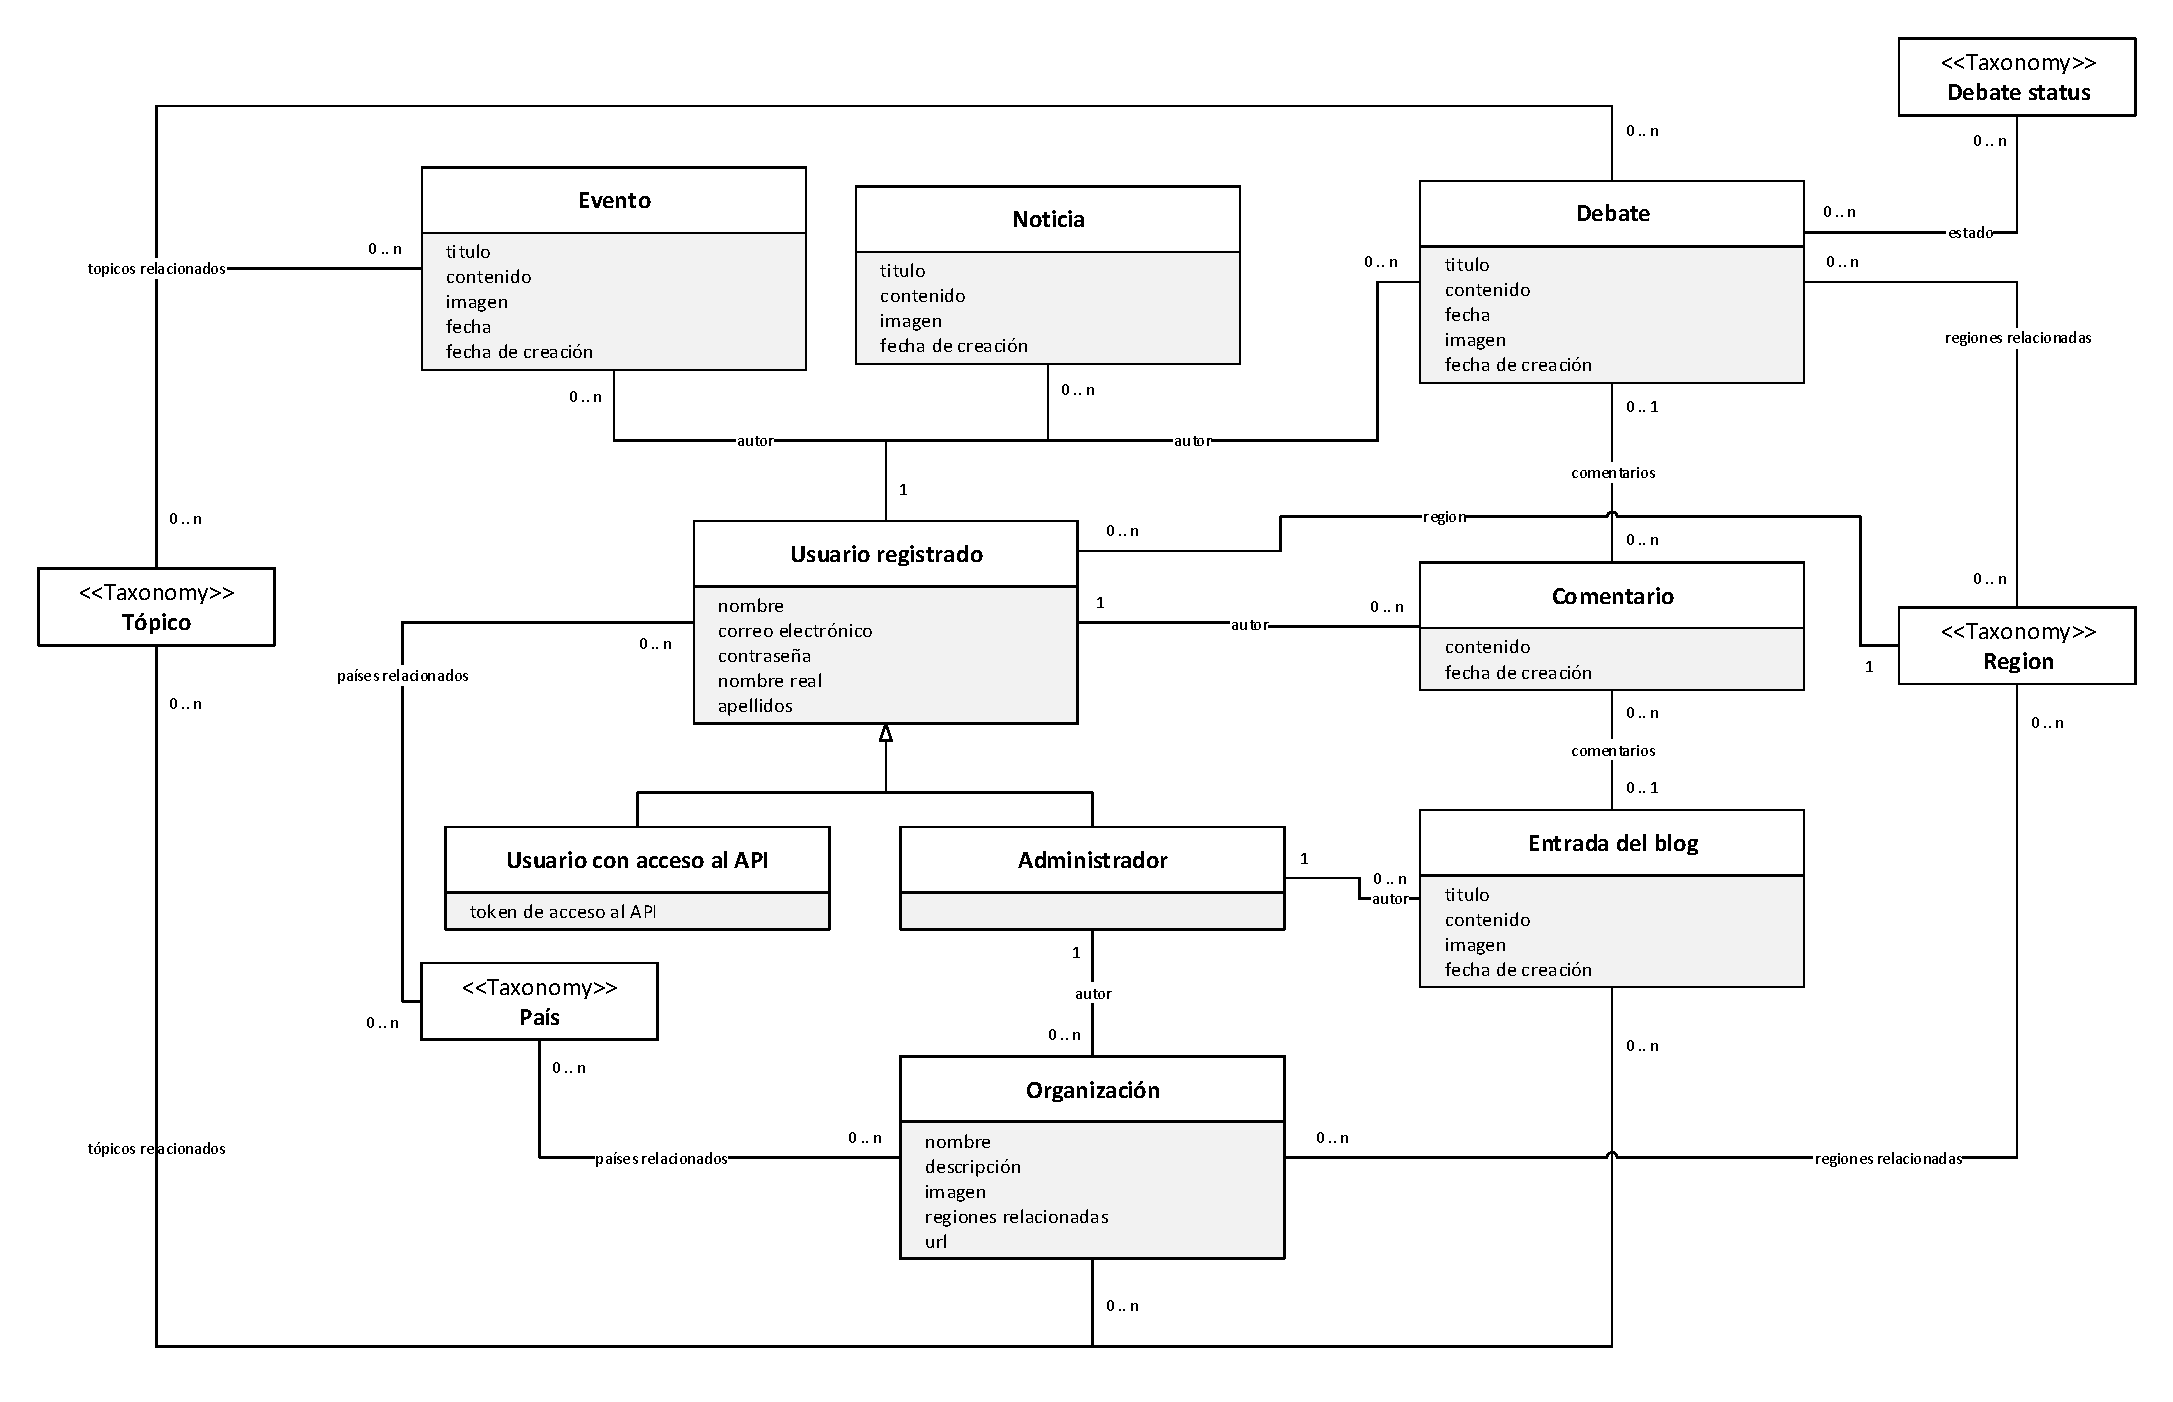
\includegraphics[width=25cm]{clases/clases_debate_final}
		\caption{Diseño final del modelo de datos de la zona social}
		\label{fig:diagrama_modelo_social_final}
	\end{figure}
\end{landscape}

La variación respecto al diseño preliminar de éste modelo que se puede observar en la sección ``\nameref{clases_preliminares_modelo_debate}'' perteneciente al capítulo \ref{chapter04} es mínima y se explicará a continuación:
\begin{itemize}
	\item Los \textbf{tópicos relacionados} de los eventos, debates, organizaciones y entradas del blog han sido extraídos a una taxonomía externa.
	\item Los \textbf{países relacionados} de las organizaciones y usuarios también han sido extraídos a una taxonomía externa.
	\item Al igual que los anteriores, las \textbf{regiones relacionadas} de las organizaciones y los debates también han sido extraídos a una taxonomía externa.
	\item El \textbf{estado} de los debates también pertenece a una taxonomía externa.
\end{itemize}

La razón principal de éstas taxonomías es la capacidad de \textit{enlazar} los diferentes contenidos del portal.  Por ejemplo, ver un elemento de la taxonomía \textit{Tópico} permitirá acceder a todos los eventos, debates, organizaciones y entradas del blog relacionados con dicho término.\\
En cuanto a los debates, la existencia de una taxonomía que represente su estado permite añadir o eliminar nuevos estados de forma sencilla y sin tener que realizar ninguna modificación en los componentes del modelo.

\subsubsection{Elementos del modelo de datos}
A pesar de la inclusión de taxonomías para representar algunos elementos del modelo de datos de la zona social, éste no ha sufrido ninguna variación respecto a lo ya expuesto en la fase de análisis del sistema. Todas las descripciones de campos y elementos realizadas en la sección ``\nameref{clases_preliminares_modelo_debate}'' del capítulo \ref{chapter04} siguen siendo válidas.


\subsection{Sistema de gestión de base de datos}
Puesto que, tal y como se explicó en las secciones ``\nameref{vista_landportal_uris}'' y ``\nameref{vista_receiver}'' pertenecientes a este mismo capítulo, el subsistema de datos está formado por dos componentes diferentes (uno de ellos incluido dentro del gestor de contenidos), se utilizarán dos aproximaciones distintas para acceder a la base de datos.

En primer lugar, el punto de entrada de datos utilizará un ORM (\textit{Mapeador Objeto-Relacional}) que actúe como intermediario con la base de datos.  De ésta forma  durante la inserción de datos no se tendrá que recurrir a realizar consultas SQL manualmente y el ORM será el encargado de persistir los nuevos objetos y actualizar el estado de los ya existentes.

Por otra parte, el framework que da soporte a la creación de visualizaciones y obtiene los datos con los que rellenar las vistas del CMS utilizará consultas manuales en lenguaje SQL.  En este caso se ha optado por la realización de consultas directamente en lenguaje SQL principalmente por la necesidad de reducir tanto el número de consultas como el número de datos innecesarios que se piden a la base de datos.  La necesidad de optimización viene dada por los grandes volúmenes de datos con los que se trabajará, teniendo lugar además estas transacciones en un momento crítico debido a que el usuario estará esperando activamente a que el sistema le muestre los datos y, por tanto, el tiempo de respuesta deberá ser el mínimo posible\footnote{Para intentar reducir aún más el tiempo de respuesta, también se utiliza un sistema de caché para evitar pedir en múltiples ocasiones los mismos datos.  El funcionamiento del caché puede consultarse en la sección ``\nameref{vista_receiver}'' del presente capítulo}.

En cuanto al sistema de gestión de bases de datos, se ha utilizado una base de datos MySQL debido a su probada estabilidad y rendimiento, además de ser la base de datos utilizada nativamente por Drupal.
